\documentclass[11pt,a4paper]{article}
\usepackage[utf8x]{inputenc}
\usepackage{graphicx}
\newcommand{\myincludegraphics}[2][]{% 
	\begingroup\setlength{\fboxsep}{0pt}% 
	\fbox{\includegraphics[#1]{#2}}% 
	\endgroup} 
\usepackage{esdiff}
\usepackage[english]{babel}
\usepackage{color}
\usepackage{booktabs}
\usepackage{tabularx}	
\usepackage{float}
\usepackage{natbib}
\usepackage{enumitem}
\usepackage{epstopdf}
\usepackage{afterpage}
\usepackage{caption}
\usepackage{subcaption}
%\captionsetup[table]{oneside , margin = {2cm, 0cm},
%	justification=RaggedRight, singlelinecheck = false }
\usepackage{subcaption}
\usepackage{mathtools}
\usepackage{multicol}
\usepackage{algorithm2e}
\usepackage{microtype}
\usepackage{titling}
\usepackage{amsmath}
\usepackage{verbatim}
\usepackage{tasks}
\usepackage[hidelinks]{hyperref} % the option is there to remove the square around links which is what I don't like.
\usepackage{comment}
\usepackage[framed,numbered,autolinebreaks,useliterate]{mcode}
\usepackage{perpage} 
\MakePerPage{footnote} % Reset the footnote counter perpage. may require to run latex twice.
\usepackage{commath} % for absolute value
\usepackage[margin=2cm]{geometry} % This is here to fit more text into the page.

\setcounter{secnumdepth}{1}  % This removes the numbering from the subsections.
% If you want the numbering of the subsection level just remove this line
\usepackage{titling}
\newcommand{\subtitle}[1]{%
	\posttitle{%
		\par\end{center}
	\begin{center}\large#1\end{center}
	\vskip0.5em}%
}

\setlength{\parindent}{0pt} % No indentation for paragraphs. Because that is just old.
\setlength{\parskip}{\baselineskip} % Instead use vertical paragraph spacing.

\fontencoding{T1} % the better font encoding.
\title {\textbf{\textsc{Exercise 12 – Digital PWM modulator}} \\[1ex] \textsc{REPORT}}
%\date{11/06/2020}
\author{Giorgio Checola}

\makeatletter
\def\@maketitle{
\graphicspath{ {./images/} }
\begin{center}
	
\includegraphics[width=75mm]{images/logoSingolo.PNG} \\
	\vspace{10mm}
	\LARGE{UNIVERSIT\`A DEGLI STUDI DI TRENTO}
	\large
	
	Department of Industrial Engineering\\
	
	
	\vspace{15mm}
	\item { \Large Master's degree in \emph{Mechatronics Engineering}}
	\vspace{3mm}			
	\item { \Large Course of Systems and techniques for digital signal processing} \\			
	
	\vspace{12mm}		
	
	\item {\huge \@title }

	\vspace{7mm}
	
	\begin{flushleft}
		\textbf{Professors:\hfill Student:} \\
		\smallskip
		David Macii \hfill Giorgio Checola \\
		Daniele Fontanelli
	\end{flushleft}
	
	\vfill
	Academic Year 2020 - 2021
	
\end{center}
}
\makeatother

\begin{document}

\graphicspath{ {./images/} }
\maketitle
\thispagestyle{empty}
\newpage
\thispagestyle{empty}
\mbox{}
\newpage


\section{Introduction}
Pulse width modulation (PWM) controller is commonly used for direct current (DC) motor control in robotics and other applications. Its switching frequency is a key parameter to reduce torque ripples and acoustic noise, and to meet the severe requirements to the power converters \cite{sato2007output}. \\
The problem is that the control resolution is inversely proportional to the switching frequency. Consequently, a higher switching frequency results in lower PWM resolution which may cause undesirable lower order harmonic components in the output current. \\
Quantization noise shaping based on $\Sigma\Delta$ modulation has been applied extensively to mitigate this problem and to improve the output waveform. $\Sigma\Delta$ operation consists in quantizing the input command (a duty cycle or a sinewave) to the low resolution of the DPWM and shaping the quantization noise. In this way it's possible to minimize requirements on its resolution. \\
As the loop integrates the error between the sampled signal and the input signal, it low-pass filters the signal and high-pass filters the noise. The differentiator factor $NTF(z)$ pushes the noise at high frequencies and converts the lower order harmonics caused by poor resolution into higher order harmonics. Then, noise and disturbance are attenuated by the output LC filter of the converter \cite{deblecker2011high}, \cite{lukic2007multibit}. \\
This report summaries the work on implementation, simulation and performance evaluation of $\Sigma\Delta$ DPWM modulators.\\
Figure \ref{buck} shows the complete electronic system considered by Norris et al \cite{norris2008quantization}. Figure \ref{model} the error-feedback configuration and a standard linear model of the system. 
\begin{figure}[H]
	\centering
	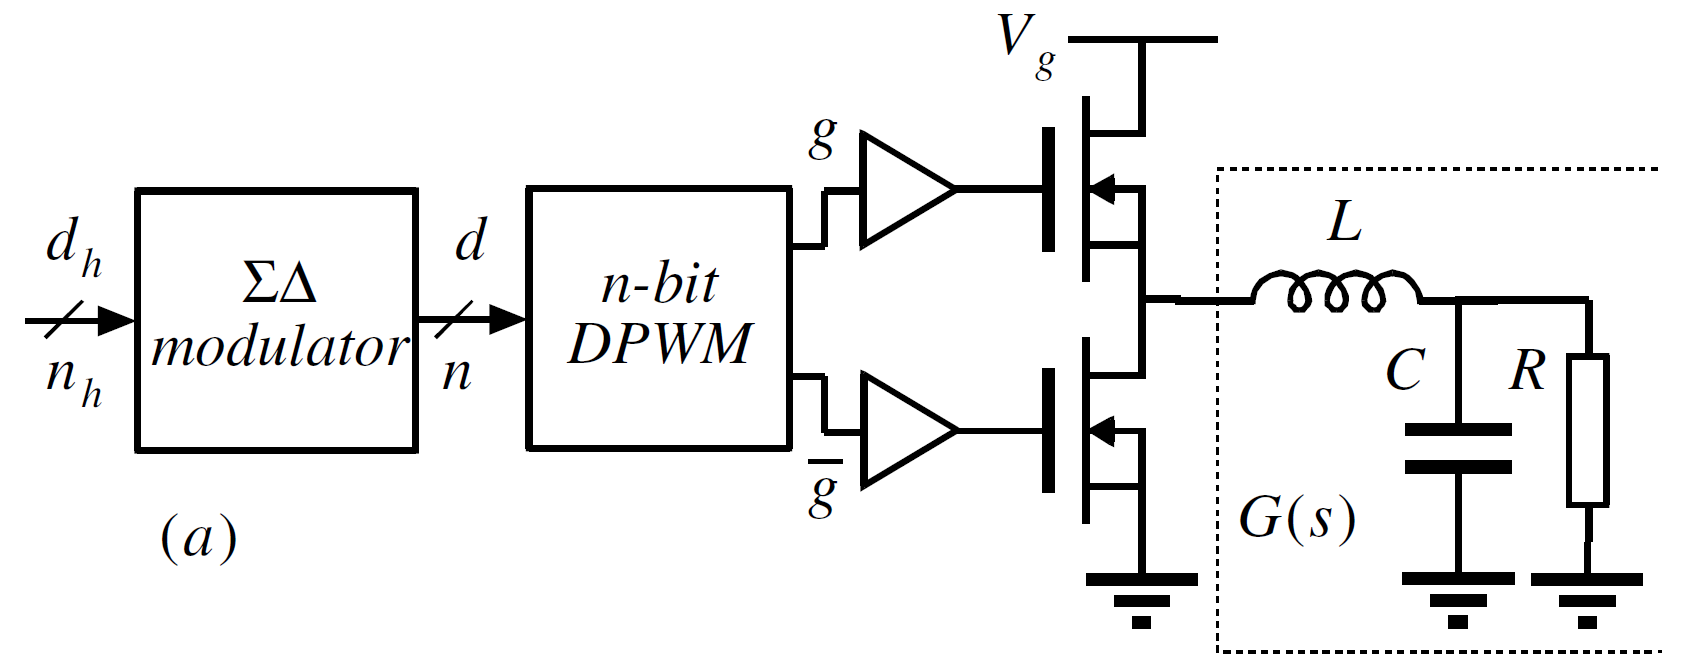
\includegraphics[width=75mm]{images/buckconverter.png}
	\caption{Digital controlled syncronous buck converter}
	\label{buck}
\end{figure}
\begin{figure}[H]
	\centering
	\begin{subfigure}[b]{0.45\textwidth}
		\centering
		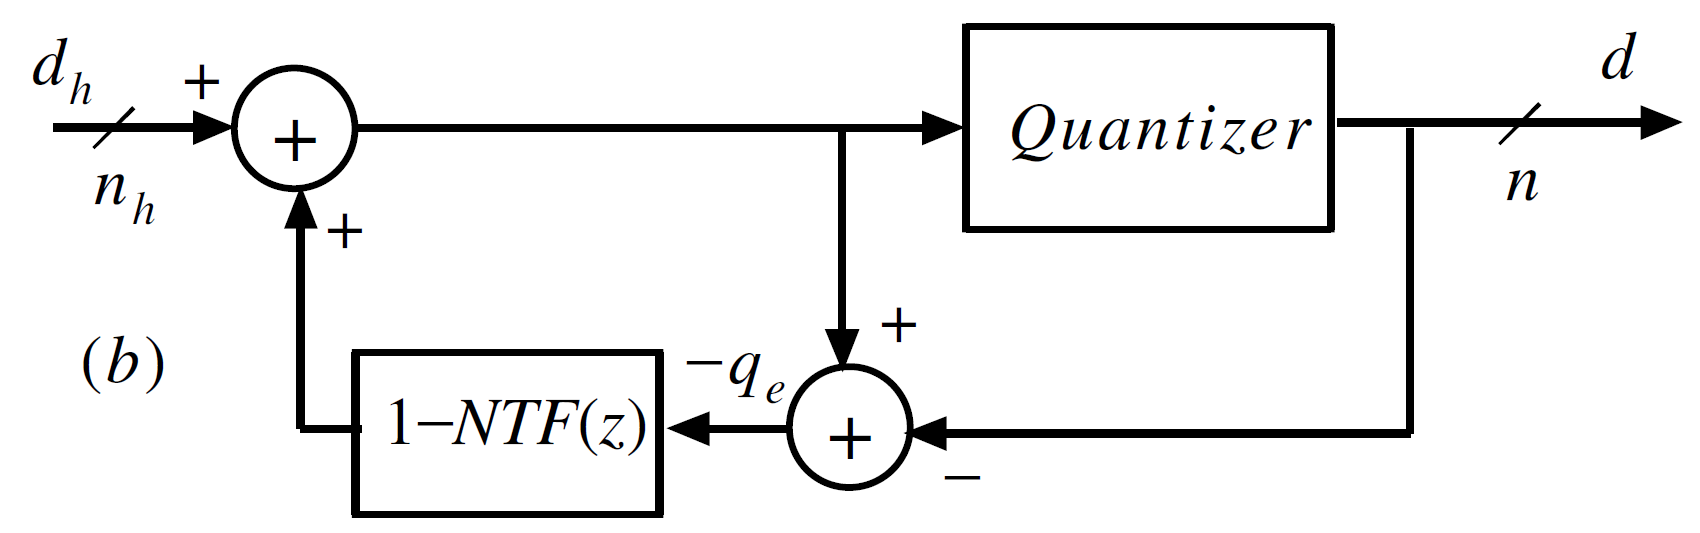
\includegraphics[width=70mm]{images/errorfeedback.png}
		\caption{Error-feedback architecture}
		\label{error}
	\end{subfigure}
	\begin{subfigure}[b]{0.45\textwidth}
		\centering
		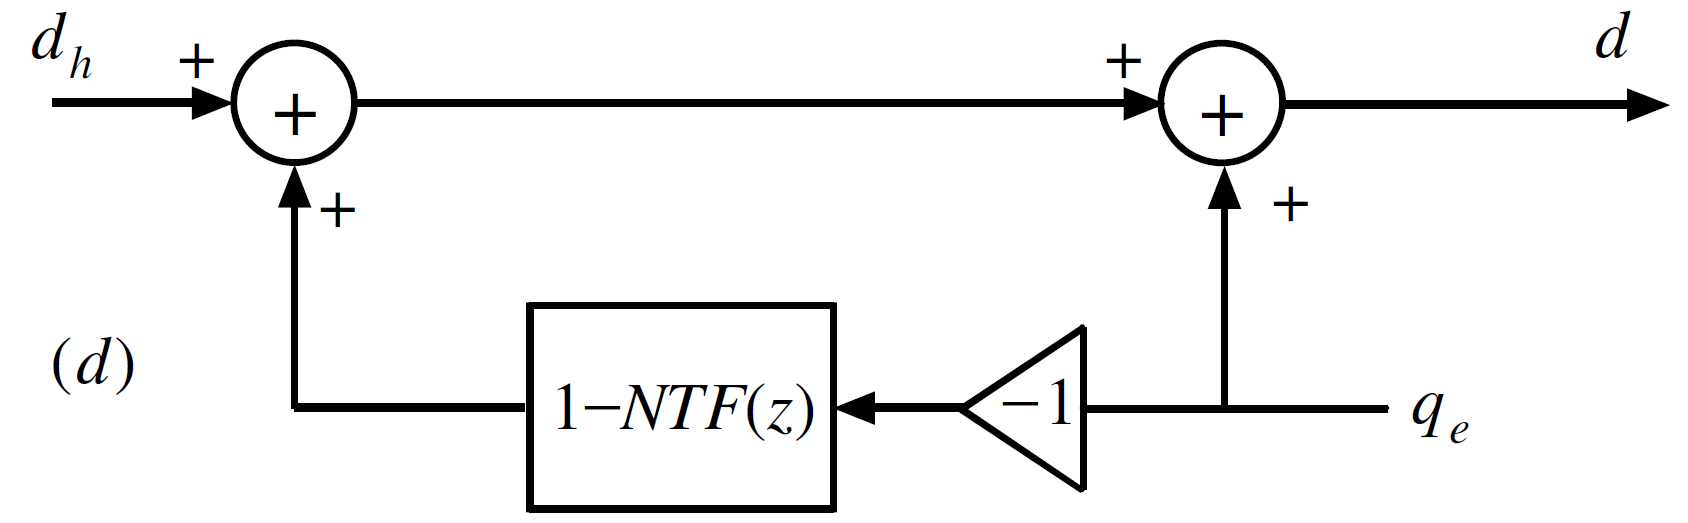
\includegraphics[width=70mm]{images/linearmodel.png}
		\caption{linear model}
		\label{linear}
	\end{subfigure}
	\caption{$\Sigma\Delta$ model}
	\label{model}
\end{figure}
The choice of the noise transfer function $NTF(z)$ is a key design consideration and determines how effectively the modulator meets the objectives of noise shaping \cite{norris2008quantization}. The table in figure \ref{table1} shows 4 classes of modulator. 
\begin{figure}[H]
	\centering
	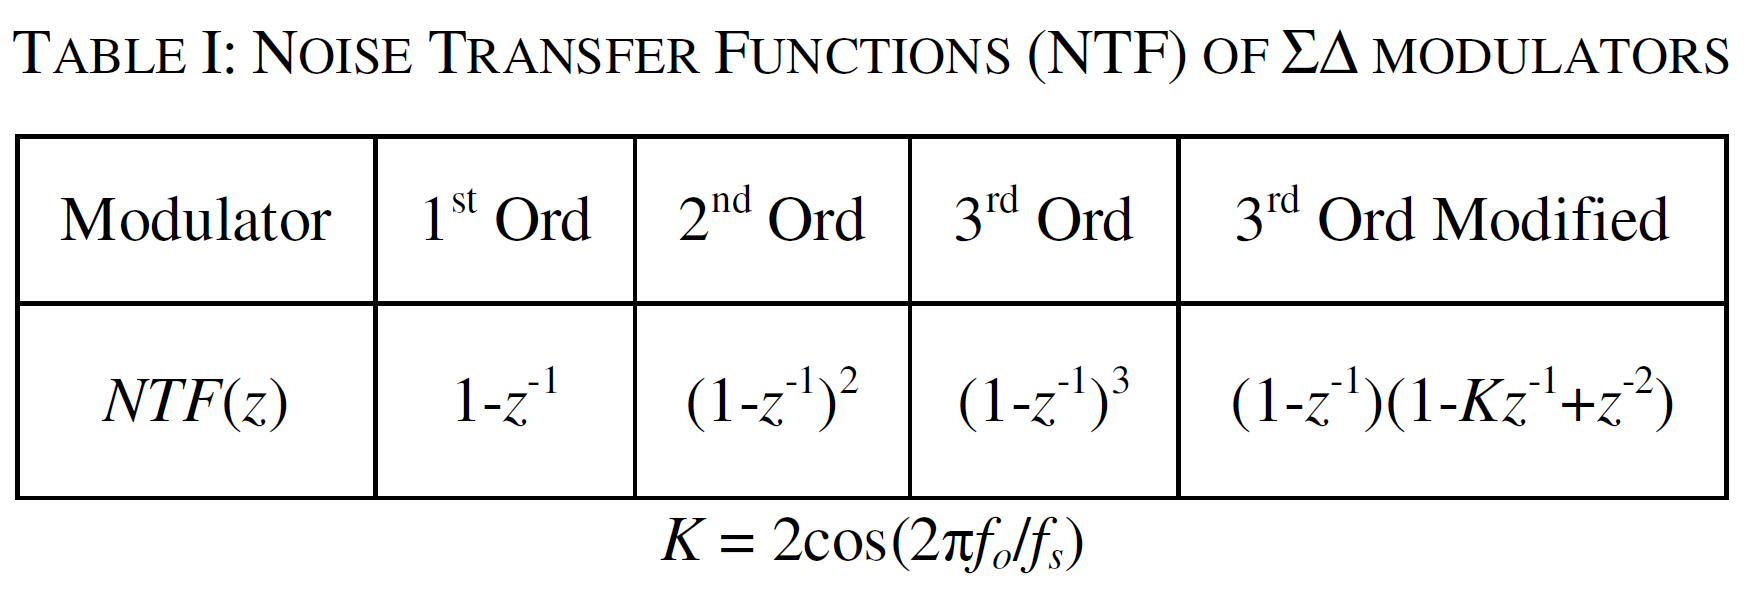
\includegraphics[width=75mm]{images/noiseshapertf.png}
	\caption{Noise transfer functions}
	\label{table1}
\end{figure}



\section{Implementation and frequency response}
I started plotting the frequency response of $\Sigma\Delta$ noise shapers. In the figure below we can see the first, second and third order, plus the third order modified and the second order buck output filter, as described in \cite{norris2008quantization}. 
For the digital filters I used the function \texttt{freqz} using the coefficients of figure \ref{table1}, while for the buck filter \texttt{freqs} with transfer function $H(s)=\frac{1}{LCs^2+Cs+1}$. 
\begin{figure}[H]
	\centering
	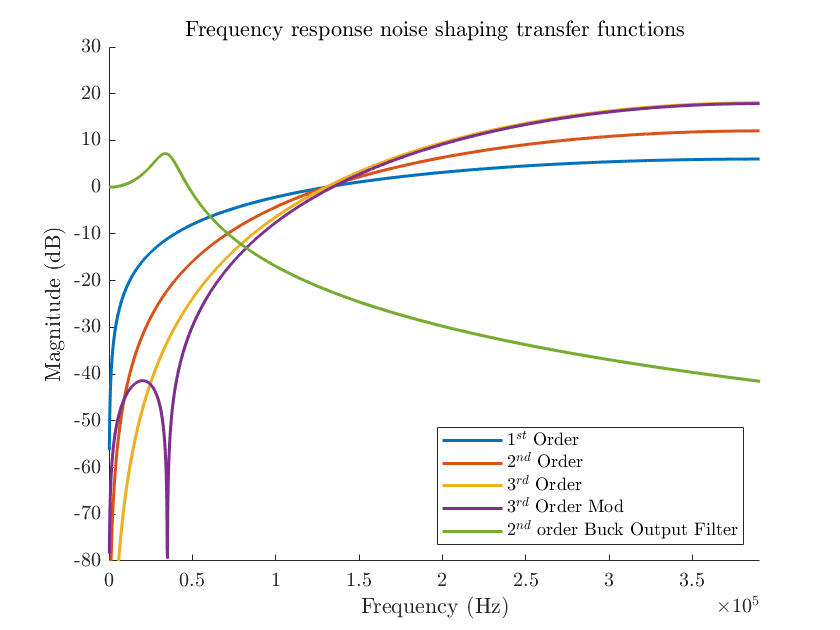
\includegraphics[width=75mm]{images/freqresp.png}
	\caption{Frequency response of the filters}
	\label{noise}
\end{figure}
All noise shapers have a zero at DC ($z=e^{j\omega}=1\rightarrow \omega=0$),  which eliminates DC output errors.

\begin{comment}
	From the linear model of the system (Fig.\ref{linear}) we obtain the following equation: 
	\begin{equation}
	d = d_h + NTF(z)q_e
	\end{equation}
	where $d_h$ is a high resolution duty cycle command and $d$ the low resolution quantized one. \\
	In Fig.\ref{noisefiltered} I displayed the power spectral density of the noise ``colored" by the noise shaper filters. Quantization noise has been modeled as white noise having RMS magnitude of $1/(2^n\sqrt{12})$.
	%As we can see, it is shaped so that there is less noise at low frequencies and more noise at high frequencies in the attenuation band of the filter. higher the orders of $\Sigma\Delta$ modulator better the shaping will be. 
	\begin{figure}[H]
	\centering
	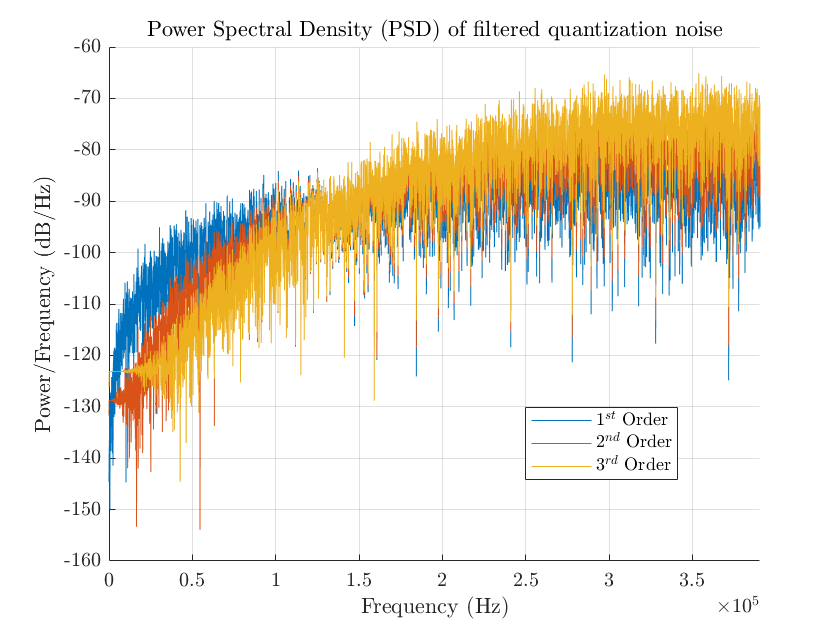
\includegraphics[width=75mm]{images/noisefiltered.png}
	\caption{$\Sigma\Delta$ Quantization noise PSD}
	\label{noisefiltered}
	\end{figure}
\end{comment}

% $\abs{NTF}=2\abs{sin\frac{\omega T}{2}}$
In order to implement a $\Sigma\Delta$ DPWM modulator, I performed a time-domain analysis based on the error-feedback architecture in figure \ref{error}. It's a very simple system loop obtainable from the inverse $Z$-transform. The quantized output $d$ is compared to the carrier of the DPWM. \\
I will show the case for the first order and leave the rest in the MATLAB code.
\begin{lstlisting}
for i = 1:length(t)
	if i == 1
		x1(i) = d_sine_sim(i);
		d1(i) = quant(x1(i), Q);
		q_e_sim1(i) = d1(i) - x1(i);
	else
		x1(i) = d_sine_sim(i) - q_e_sim1(i-1);
		d1(i) = quant(x1(i), Q);
		q_e_sim1(i) = d1(i) - x1(i);
	end
end
	
for i = 1:1:length(t)
	if car_q(i) <= d1(i)  
		pwm1(i)=1;
	else
		pwm1(i)=0;
	end
end
\end{lstlisting}
As input, \texttt{d\_sine\_sim}, I used a sinusoidal reference signal with fundamental frequency of 300 Hz and amplitude $A=0.8$, while for the DPWM carrier a triangular wave with switching frequency of 50 kHz, quantized with quantization step $Q=2/2^4$. Sampling frequency $f=1$ MHz and simulation time $T_{sim}=5$ $ms$. Fig.\ref{system} shows the signal changes through the three noise shapers.
This additional noise, which increase with the order of the system, allows to reconstruct perfectly the quantized output after passing through the converter output filter ($f_0=35$ kHz), unlike in the case without shaping.
\begin{figure}[H]
	\begin{subfigure}[b]{0.3\textwidth}
		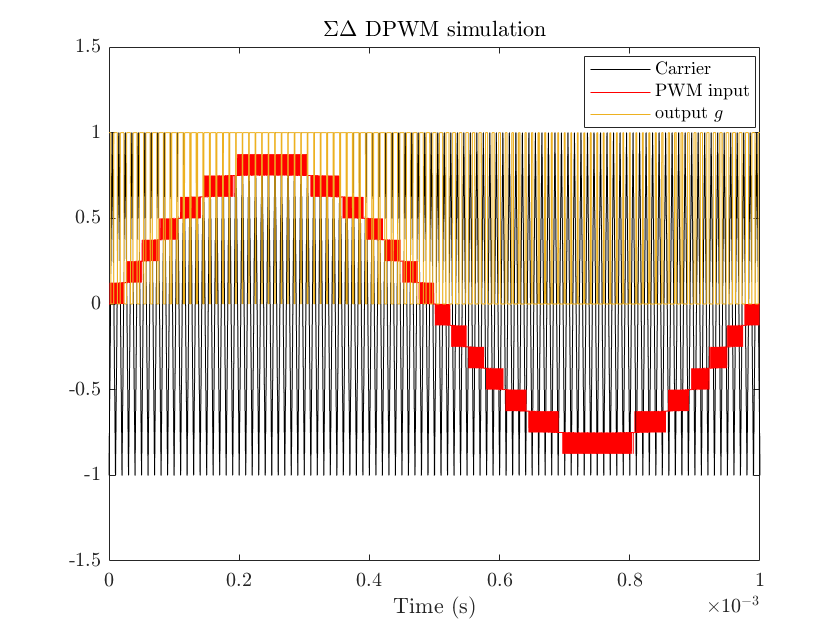
\includegraphics[width=50mm]{images/simulation1order.png}
		\caption{$1^{st}$ order}
	\end{subfigure}
	\hfill
	\begin{subfigure}[b]{0.3\textwidth}
		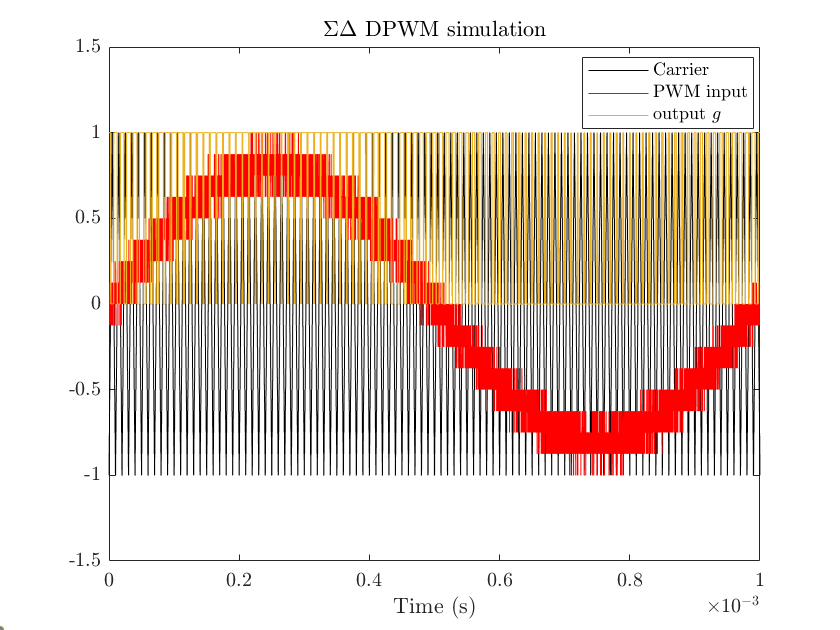
\includegraphics[width=50mm]{images/simulation2order.png}
		\caption{$2^{st}$ order}
	\end{subfigure}
	\hfill
	\begin{subfigure}[b]{0.3\textwidth}
		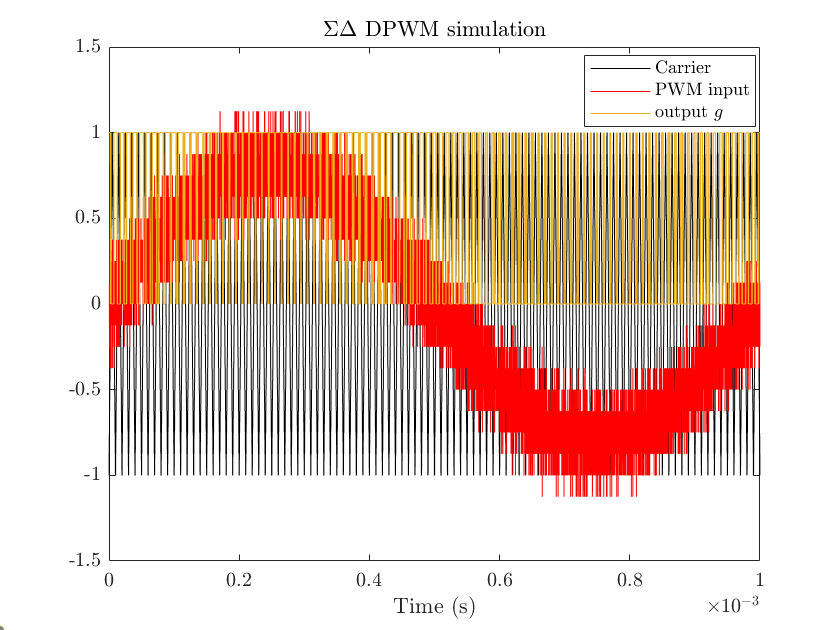
\includegraphics[width=50mm]{images/simulation3order.png}
		\caption{$3^{st}$ order}
	\end{subfigure}
	\caption{$\Sigma\Delta$ DPWM signals}
	\label{system}
\end{figure}

\begin{figure}[H]
	\centering
	\begin{subfigure}[b]{0.45\textwidth}
		\centering
		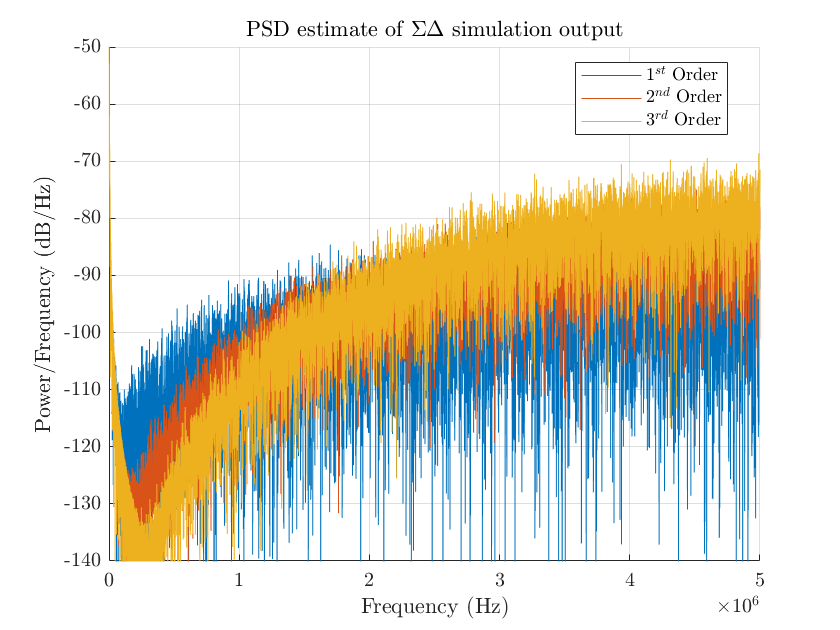
\includegraphics[width=70mm]{images/psd_d_sim.png}
		\caption{PSD of $\Sigma\Delta$ simulation output}
		\label{sim}
	\end{subfigure}
	\begin{subfigure}[b]{0.45\textwidth}
		\centering
		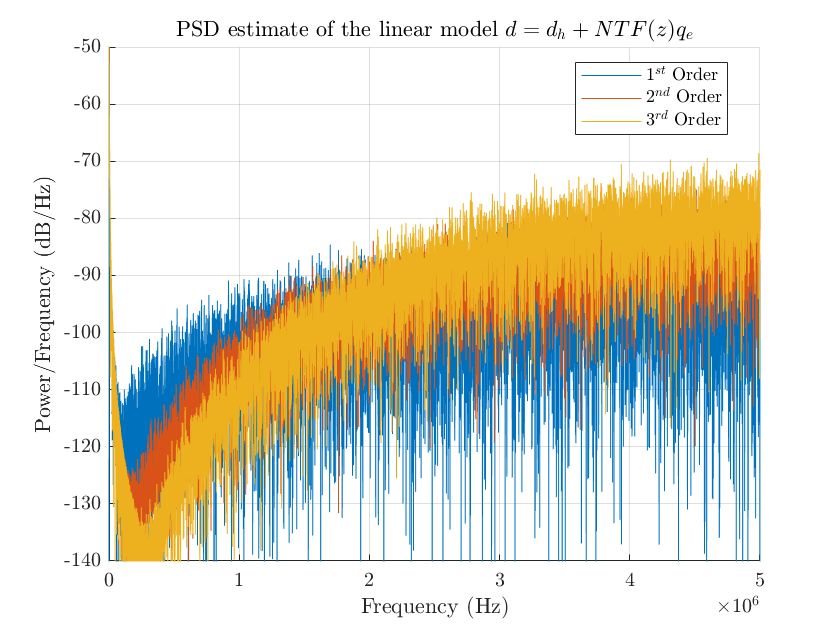
\includegraphics[width=70mm]{images/psd_linmodel.png}
		\caption{PSD of $\Sigma\Delta$ linear model output}
		\label{lin}
	\end{subfigure}
	\caption{Comparison of $\Sigma\Delta$ output PSD}
	\label{psd comparison}
\end{figure}
The figure above shows a comparison between the PSD of the output $d$, obtained from the simulation in time-domain, and by using the linear model of Fig.\ref{linear}. It's visible the reduction of noise power at low frequencies, and the increase at high frequencies for higher order systems. The correctness of the implementation is confirmed by the identical spectral components of $\Sigma\Delta$ output and linear model.
\section{Performance evaluation}
We can test the various $\Sigma\Delta$ architectures in terms of signal-to-noise and distortion ratio (SINAD) and total harmonic distortion (THD). The reason is that DPWM sampling results in signal distortion affecting the noise-shaping performance. Moreover its non-linearity adds distortion which ends up moving back some noise from high to low frequencies \cite{norris2008quantization}, \cite{sato2007output}.

SINAD is a measure of the quality of a signal. It's the ratio between the total received power and the noise-plus-distortion power. Total harmonic distortion (THD) is a measurement of the distortion that an electronic device introduces in a signal which passes through, and depends on the amplitude of the harmonics.
%A SINAD value of 12 dB is the ``standard value". Higher values correspond to better audio quality. 
Normally, we could compute this value manually, but in this case, since it cannot be measured directly due to quantization and PWM non linear function, we need to do an estimation using periodogram analysis. This is done with the function \texttt{sinad} and \texttt{thd}. \\
I started by plotting the power spectrum of the quantized output $d$ and the pulsating DPWM outputs $g$ (Fig.\ref{spectrum}). \\
In the left figure we can see the characteristic behavior due to the noise transfer function $NTF(z)$ and the case without shaping, in which noise is high at low frequencies and lower at higher ones. In the figure on the right, instead, the spectra after passing through the staircase PWM function. The output $g$ is a square wave made up of multiple harmonics summed together. The visible peaks are situated at the fundamental frequency (50 kHz) and at its higher harmonics. By going up with the orders of $\Sigma\Delta$, noise power increases at high frequencies, while peaks are slightly lowered at small frequencies. 
\begin{figure}[H]
	\centering
	\begin{subfigure}[b]{0.45\textwidth}
		\centering
		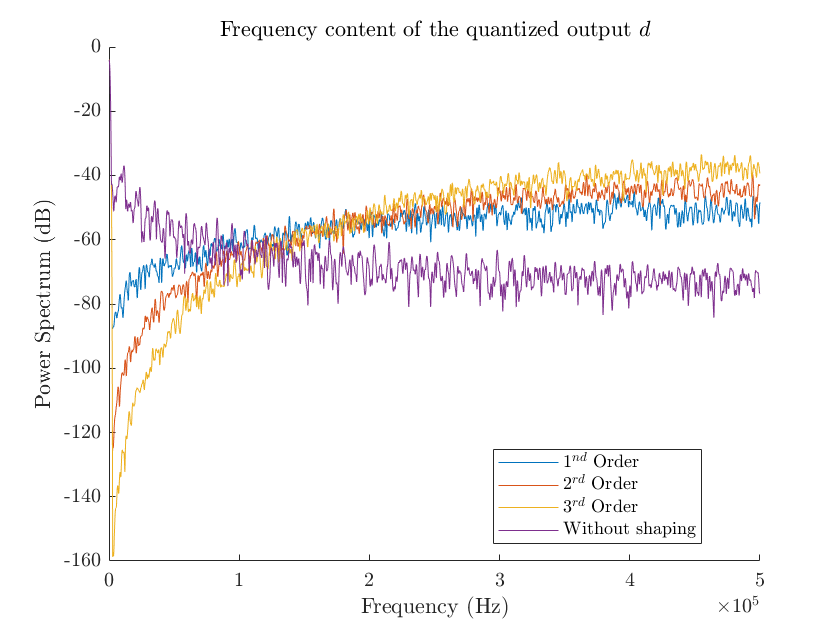
\includegraphics[width=70mm]{images/powerspect_d.png}
		\caption{Power spectrum of $d$}
		\label{d}
	\end{subfigure}
	\begin{subfigure}[b]{0.45\textwidth}
		\centering
		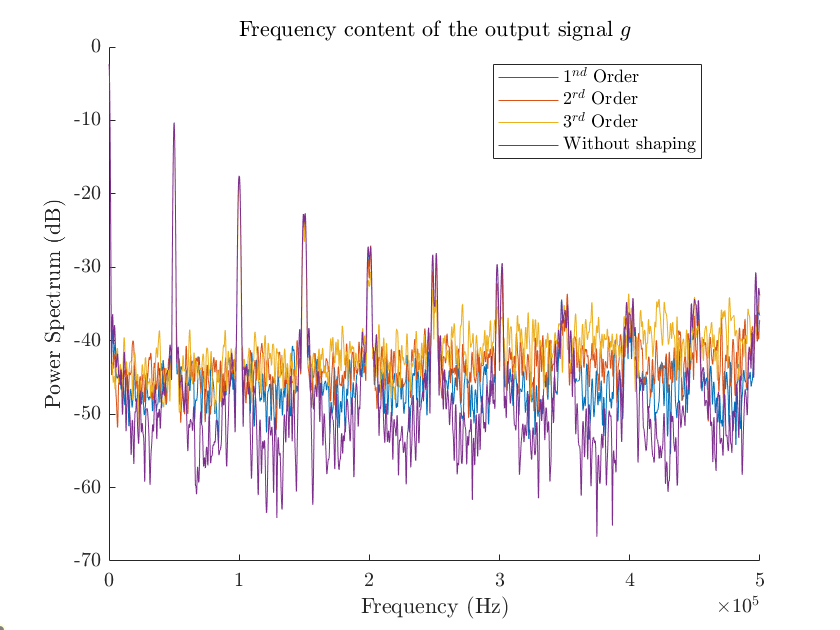
\includegraphics[width=70mm]{images/powerspect_g.png}
		\caption{Power spectrum of $g$}
		\label{g}
	\end{subfigure}
	\caption{Power spectrum of the main signals of the system}
	\label{spectrum}
\end{figure}

At this point, I analyzed the final outputs.
%\begin{table}[H]
%\centering
%	\begin{tabular}{c|c|c} 
%		\centering{$\Sigma\Delta$} & \centering{SINAD} & THD \\
%		\hline
%		Carrier& $18$ dB & $-18$ dB  \\
%		$d$ without shaping & $24$ dB & $-34$ dB \\
%		$d_1$ & $20$ dB & $-66$ dB \\ 
%		$d_2$ & $16$ dB & $-96$ dB \\ 
%		$d_3$ & $10$ dB & $<-100$ dB \\ 
%	\end{tabular}
%\caption{SINAD and THD values before DPWM}
%\label{t1}
%\end{table}
\\
My best results in term of SINAD and THD were achieved by considering the periodogram power spectrum estimate, by reducing the number of DFT points to 1000 and 500 respectively, and using a hanning window. They were chosen after a process of trial and error varying several settings. Moreover I had to neglect sampling frequency to compute SINAD. All values are listed in Table \ref{t2}.
\begin{table}[H]
	\centering
	\begin{tabular}{c|c|c} 
		\centering{$\Sigma\Delta$ DPWM} & \centering{SINAD} & THD \\
		\hline
		Carrier& $18$ dB & $-18$ dB  \\
		Without shaping& 30.64 dB & -11.86 dB  \\
		$1^{st}$ order & 30.47 dB & -12.50 dB \\
		$2^{nd}$ order & 30.46 dB & -13.94 dB \\ 
		$3^{rd}$ order & 30.05 dB & -14.77 dB \\ 
	\end{tabular}
\caption{SINAD and THD values after DPWM}
\label{t2}
\end{table}
Results shows that signal-to-noise and distortion ratio does not change with the order of the system, while total harmonic distortion improves. This confirms the capability of $\Sigma\Delta$ modulation to limit the distortion caused by DPWM. Instead it's natural that SINAD remains constant: quantization noise is not cancelled, but it's only moved to higher frequencies. The figures below displays the frequency content of  $3^{rd}$-order $\Sigma\Delta$ output with the corresponding parameter values.
\begin{figure}[H]
	\centering
	\begin{subfigure}[b]{0.45\textwidth}
		\centering
		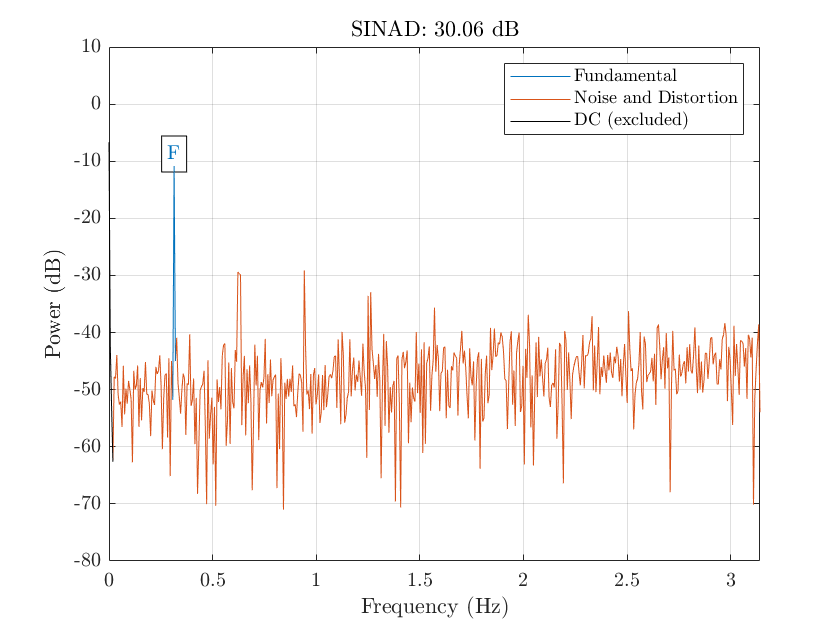
\includegraphics[width=70mm]{images/sinad3order.png}
		\label{sinad3}
	\end{subfigure}
	\begin{subfigure}[b]{0.45\textwidth}
		\centering
		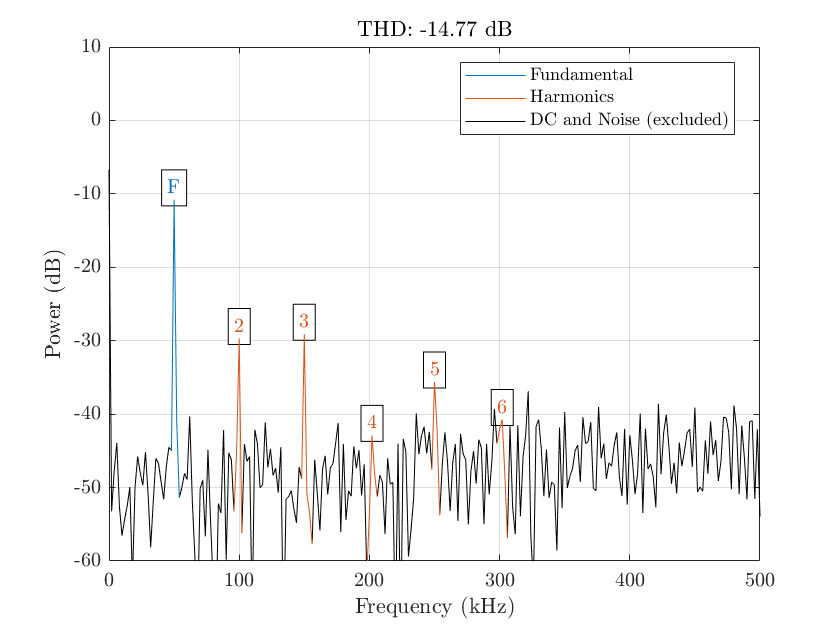
\includegraphics[width=70mm]{images/pwm3thd.png}
		\label{thd3}
	\end{subfigure}
	\caption{SINAD and THD of $3^{rd}$ order $\Sigma\Delta$ DPWM output}
	\label{sinadthd}
\end{figure}

\begin{comment}
Starting from the sinewave input and the sawtooth carrier, I noted that fundamental frequency and simulation time does not influence significantly their noise and distortion, but more the $\Sigma\Delta$ and DPWM output. In fact, higher the fundamental frequency of PWM, bigger low order harmonics are generated. \\
For what concerns $\Sigma\Delta$ quantized outputs, values improve in terms of total harmonic distortion, while decrease a little in SINAD, because of the noise power after quantization (see Fig.\ref{system}). Best results are obstained with the hamming and hanning window and number of DFT points equal to 2500 and 1000. 
\begin{figure}[H]
\centering
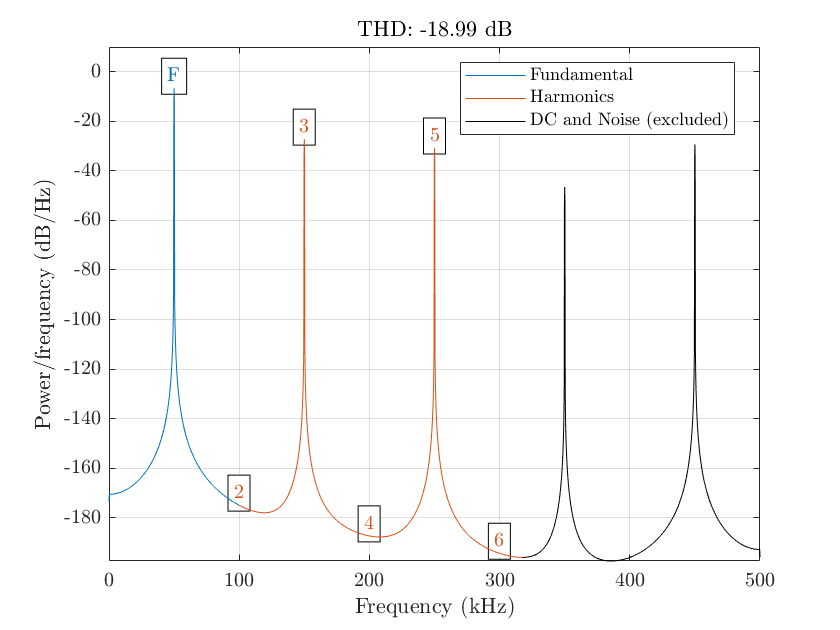
\includegraphics[width=90mm]{images/thdcarrier.png}
\caption{Total harmonic distortion of $3^{rd}$ order $\Sigma\Delta$ DPWM output}
\label{thdcar}
\end{figure}
\end{comment}
\section{Conclusions}
In this report $\Sigma\Delta$ modulators followed by discrete PWM are examined. After a small introduction about its functioning, I described the implementation of the three systems and compared them to each other.
Lastly, I computed SINAD and THD to validate their performances. For this purpose spectral estimation was necessary. \\
By trying many design choices, I noted that signal settings affect a lot the spectral content which directly changes the final value. For example: the type of input signal and its fundamental frequency, switching frequency of the carrier, the type of window functions or the numbers of DFT points over which PSD is estimated.\\
In the end SINAD remains almost constant for all the system, while THD gets better (it becomes more negative) with higher orders confirming the functionality of this architecture. 

 
\footnotesize
\newpage
\hypersetup{linkcolor = black}
\listoffigures
\listoftables
\bibliographystyle{plain}
\bibliography{bibliography}
\end{document}